\section{Zielsetzung}
\label{sec:Zielsetzung}
In diesem Versuch sollen die Kerspins der $\ce{^87Rb}$- und $\ce{^85Rb}$-Isotope
bestimmt werden. Dafür wird durch Bestrahlung mit zirkular polarisiertem Licht 
eine Besetzungsinversion erzeugt. Durch Anlegen eines Magnetfeldes wird dabei eine 
Zeemanaufspaltung realisiert. Aus der Energiedifferenz der Zeemannniveaus können bei 
bekanntem Magnetfeld und bekannter Frequenz aus dem Landefaktor die Kernspins
berechnet werden. 

\section{Theorie}
\label{sec:Theorie}

Der Versuch basiert auf dem Phänomen des sogennanten optischen Pumpens. 
Dabei wird ausgenutzt, dass Gas welches mit Licht einer passenden Frequenz 
(Differenz der angestrebten Energieniveaus) bestrahlt wird in einen Zustand 
gebracht werden kann, indem die Anzahl höhere Energiezustände über der 
Gleichgewichtskonfiguration liegt. Die Elektronenhülle der Atome 
absorbiert dabei das eingestrahlte Licht, welches das entsprechende Elektron 
auf ein höheres Energieniveau anhebt, wobei spezielle Auswahlregeln beachtet 
werden müssen.
Ohne äußere Bestrahlung ist das Verhältnis der Besetzungszahlen zweier Niveaus 
über eine Boltzmannverteilung auszudrücken und durch
\begin{equation}
    \frac{N_2}{N_1}=\frac{g_2}{g_1}\frac{\exp\left(-\sfrac{W_2}{\symup{k_B}T}\right)}{\exp(-\sfrac{W_1}{\symup{k_B}T})}
    \label{eq1}
\end{equation}
gegeben. In dieser Gleichung beschreibt $W_i$ die Energien der Zustände, 
$g_{\symup{i}}$ die Landefaktoren und $T$ die Temperatur.
Das in diesem Versuch betrachtete Gas besteht aus den Rubidiumiosotopen 
$\ce{^87Rb}$ und $\ce{^85Rb}$, wobei der Anteil von $\ce{^85Rb}$ am natürlichen 
Vorkommen 72,17\% beträgt, während der Anteil des Isoptopes $\ce{^87Rb}$
nur auf einen Prozentsatz  von 27,83\% kommt \cite{RbVorkommen}.
Rubidium gehört zur Elementenkategorie der Alkalimetalle, welche durch ihre 
Eigenschaft ein Elektron auf der äußersten Schale (s-Orbital) zu besitzen, 
charakterisiert sind.
Rubidium steht an der 37. Stelle im Periodensystem. Das bedeutet die 
Neutronenzahl von $\ce{^87Rb}$ ist 50 und $\ce{^85Rb}$ besitzt die Neutronenzahl 48.

\subsection{Quantenzahlen}

Jeder Zustand eines Fermions im Atom kann durch spezifische Quantenzahlen 
charakterisiert werden. Es werden zunächst die Fermionen der Atomhülle, also die 
Elektronen betrachtet. Die Atomhülle sei zunächst aus Hauptschalen aufgebaut die 
durch die Hauptquantenzahl $n = 1,2,3..$ benannt sind. Jede Hauptschale $n$ besitzt 
ebenfalls $n$  Unterschalen, die durch die Nebenquantenzahlen $l = 0,...,n-1$ 
indiziert werden. Jede Unterschale ist durch eine weitere Quantenzahl, 
die magnetische Quantenzahl $m_{\text{l}}=-l,...l$ substrukturiert. 
Der Spin bzw. die Spinquantenzahl der Fermionen beträgt $+\frac{1}{2}$ oder 
$-\frac{1}{2}$.
Zwei Elektronen dürfen sich nach dem Pauli-Prinzip nur dann in einem Zustand aufhalten, 
der durch die selben $n$, $l$ und $m_{\text{l}}$ definiert ist, wenn sie sich im 
Spin unterscheiden. Die Belegung der möglichen Zustände wird vom niedrigsten Energieniveau 
ausgehend begonnen und aufsteigend fortgesetzt, wobei Zustände gleicher Energie erst einfach 
und dann doppelt belegt werden.
Der Gesamtspin und der Gesamtbahndrehimuls einer Elektronenhülle ergibt sich dann 
als Summe über alle Einzelspins bzw. -bahndrehimpulse, wobei sich biede maximieren.
Das führt dazu, dass volle Haupt- und Nebenschalen nicht zu den Gesamtergebnissen 
beitragen. Der Gesamtdrehimpuls der Hülle ergibt sich aus Addition des Gesamtspins mit 
dem Gesamtdrehimpuls. Das bedeutet für die Quantenzahl des Gesamtdrehimpulses gilt 
für weniger als halbvolle Schalen $J = |L-S|$ und für mehr als halbvolle Schalen 
$J = L+S$ und für halbvolle Schalen $J(L=0) = S$. 
Der Gesamtdrehimpuls des Atomkerns wird Kernspin $I$ genannt. Der Gesamtdrehimpuls 
jedes Nukleons ergibt sich aus der Addition seines Bahndrehimpulses und Spins, 
wobei Nukleonen Fermionen sind und somit ebenfalls einen Spin von  $+\frac{1}{2}$ oder 
$-\frac{1}{2}$ besitzen können. Der Kernspin ergibt sich schließlich als Summe über die 
Drehimpulse aller Nukleonen. Die Spins der Nueonen richten sich möglichst energiearm 
aus. D.h. es tun sich immer zwei Nukleonen gleicher Art und entgegengesetzten Spins 
zusammen. Diese Paare tragen dann nicht mehr bei. Für den Fall einer ungeraden Massenzahl 
sind die Kerspins halbzahlig. So zeigt es sich, dass
$\ce{^87Rb}$ einen Kernspin von $I = \frac{3}{2}$ und  $\ce{^85Rb}$ einen Kernspin von 
$I = \frac{5}{2}$ besitzt.
Der Gesamtdrehimpuls des gesamten Atoms kann mehere Werte annehmen, die mit
$F = |J-I|, |J-I|+1,..., J+I -1, J+1$ entartet sind \cite{1}. 

\subsection{Landefaktoren}

Die Drehimpulse besitzen magnetische Momente, die als 
\begin{equation}
    \mu_{\text{J}} = \mu_{\text{B}} g_{\text{J}} \sqrt{J(J+1)}
\end{equation}
für den Gesamtdrehimpuls der Elektronenhülle bzw. als 
\begin{equation}
    \mu_{\text{I}} = \mu_{\text{B}} g_{\text{I}} \sqrt{I(I+1)}
\end{equation}
für das magnetische Moment des Kerns gegeben sind.
Für den Gesamtdrehimpuls folgt analog das magnetische Moment 
\begin{equation}
    \mu_{\text{F}} = \mu_{\text{B}} g_{\text{F}} \sqrt{F(F+1)}
\end{equation}
des gesamten Atoms \cite{1}.
Die Faktoren $g_{\text{i}}$ werden als Landefaktoren bezeichnet.
So zeigt sich, dass der Landefaktor $g_{\text{J}}$
als 
\begin{equation}
    g_{\text{J}} = 1+ \frac{J(J+1) +S(S+1) -L(L+1)}{2J(J+1)}
\end{equation}
gegeben ist.
In diesem Versuch  ist der Landefaktor $g_{\text{F}}$ von Bedeutung, da
aus ihm der Kernspin bestimmt werden kann. 
Er ist durch die Formel
\begin{equation}
    g_{\text{F}} = g_{\text{J}} \frac{F(F+1) + J(J+1) - I(I+1)}{2F(F+1)} 
\end{equation}
gegeben \cite{2}. 

\subsection{Zeemanaufspaltung} 

Der Zeemaneffekt ist ein physikalisches Phänomen, dass die Aufspaltung von
Spektrallinien aufgrund eines äußeren Magnetfeldes beschreibt. Die Ursache dieses 
Effektes ist über die Wechselwirkung des äußeren Magnetfeldes mit den magnetischen 
Momenten der Atombestandteile zu erklären. Diese Wechselwirkung führt zu 
Verschiebeungen der Energieniveaus, bzw. in eine Aufspaltung eines ursprünglichen 
Niveaus in eine bestimmte Anzahl äquidistanter Unterniveaus (Zeeman-Nivaus). 
Ist das angelegte Magnetfeld kleiner als die Kopplung zwischen Hüllengesamtspin 
und Gesamtbahndrehimpuls der Hülle, so wird jedes Niveau mit 
Gesamtdrehimpuls $J$ in $m_{\text{J}}= -J,...,J$ Unterniveaus aufgespalten, deren 
Energiedifferenzen
\begin{equation}
    \Delta E_{\text{J}} = g_{\text{J}} \mu_{\text{B}} B m_{\text{J}}
\end{equation}
betragen. Für diesen Fall wird dann von einer Aufspaltung der Feinstruktur ggesprochen \cite{1}.
Wenn die Wechsewlwirkung zwischen den Drehimpulsen der Hülle und denen des Kerns 
mit in Betracht gezogen wird, dann wird von einer Aufspaltung in der Hyperfeinstruktur
gesprochen. Die Energiedifferenzen lassen sich dann über die Gleichung 
\begin{equation}
    \Delta E_{\text{F}} = g_{\text{F}} \mu_{\text{B}} B m_{\text{F}}
\end{equation}
ausdrücken, wobei $m_{\text{F}}$ die Werte $-F,...,F$ annehmen kann.
Das heißt, ein Niveau mit Quantenzahl $F$ spaltet sich in $2F+1$ Unterniveaus auf \cite{2}.
Eine Skizze dieser Aufspaltung ist in in der folgenden Abbildung für 
die Rubidiumiostope dagestellt.
\begin{figure}
    \centering
    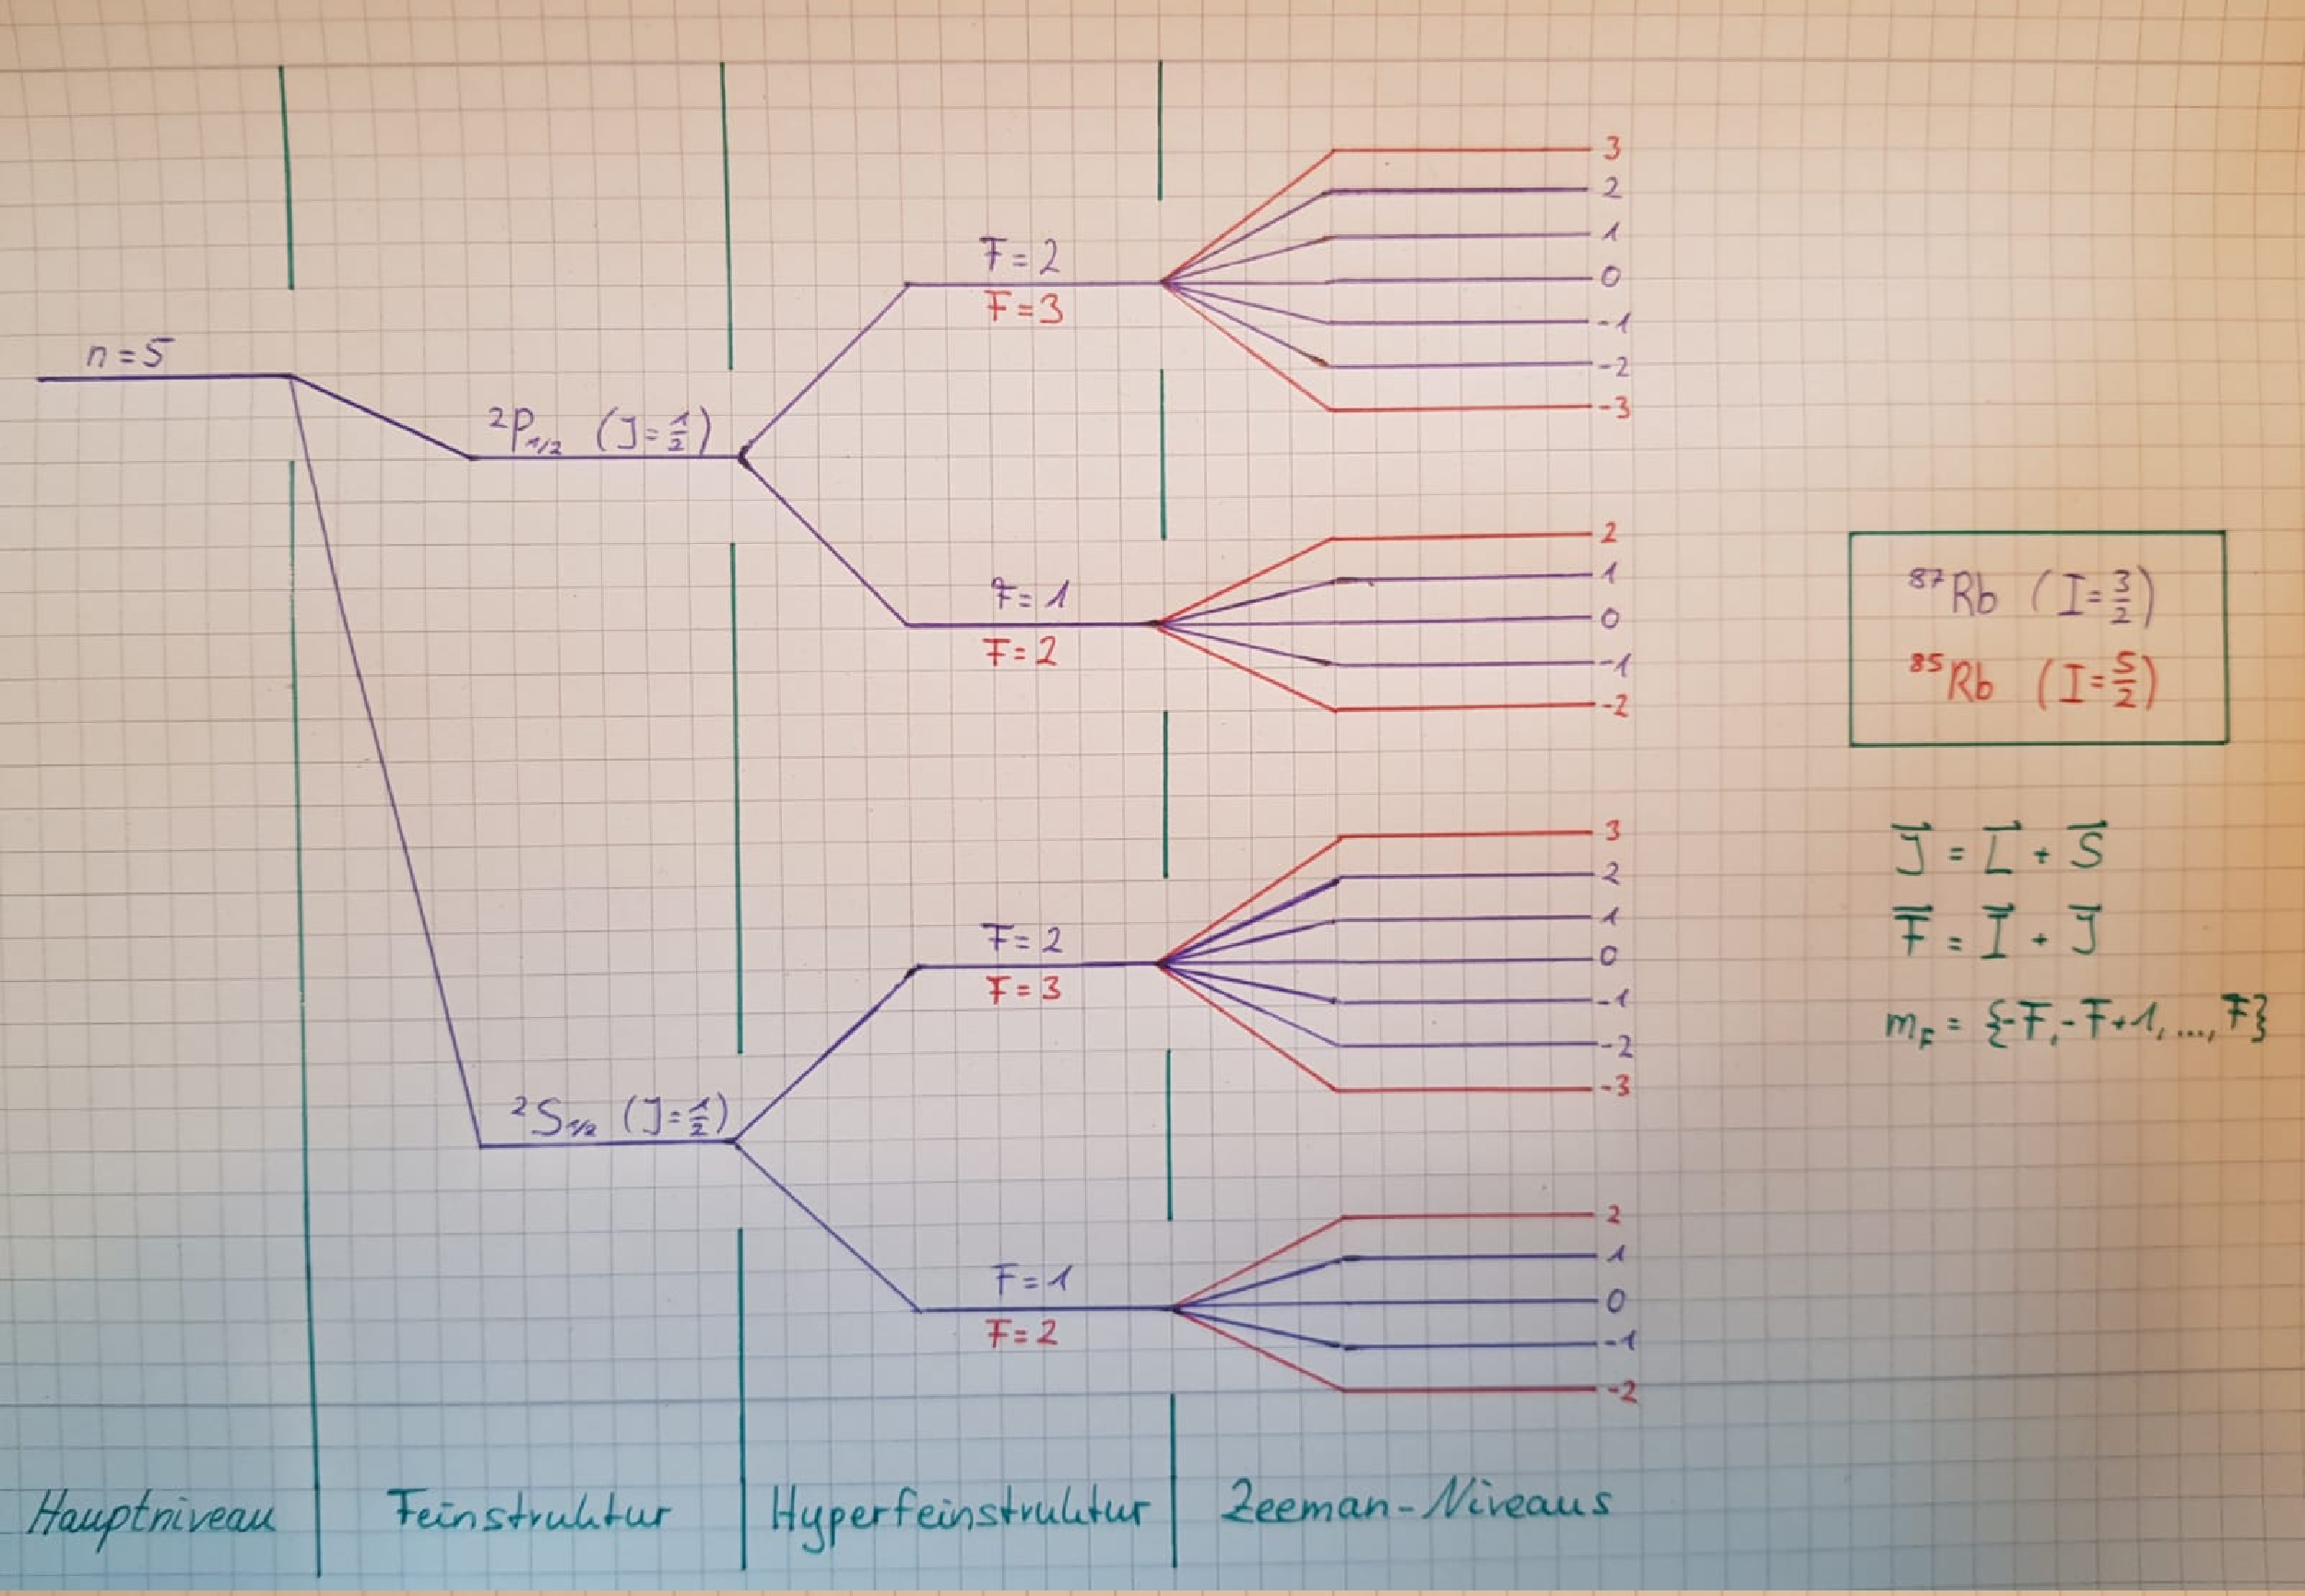
\includegraphics[width=0.8\textwidth]{figure/Zeemanniveaus.pdf}
    \caption{Auf dieser Abbildung ist die Hyperfeinstrukturaufspaltung der 
    verwendeten Rubidiumiostope zusehen.}
    \label{abb1}
\end{figure}

\subsection{optisches Pumpen}

Das Ziel des optischen Pumpnes ist, das Gas aus seinen thermisch, gleichgewichtig
verteilten
Besetzungszuständen in einen Zustand zu bringen, bei dem die Anzahl der höherenergetischen 
Besetzungszuständen gegenüber den Niederenegetischen überwiegt. Bei einem 
entsprechend angeregten System, wird auch von Besetzungsinversion gesprochen.
Durch Einstrahlung von Licht, dessen Energie der Differenz der Niveaus 
$\ce{^{2}S_{\frac{1}{2}}}$ und $\ce{^{2}P_{\frac{1}{2}}}$ entspricht,
können Elektronen durch Absorption dieser Wellen vom Niveau 
$\ce{^{2}S_{\frac{1}{2}}}$ in das Niveau $\ce{^{2}P_{\frac{1}{2}}}$ übergehen,
wenn sie den Auswahlregeln genügen.
Die Auswahlregeln sind durch die Relationen
\begin{equation}
    \Delta l = \pm 1 \qquad \Delta m = 0, \pm1
\end{equation}
gegeben. In diesem Fall gilt $m = m_{\text{F}}$, sodass ein Übergang bei passender 
Frequenz nur möglich ist, wenn die Differenz der Quantenzahlen $m_{\text{F}}$ 
von Ausgangs- und Endzustand $0$ oder $\pm 1$ beträgt und die Differenz der 
Quantenzahl $l$ einen Betrag von $1$ aufweist. Zweiteres ist bei Übergängen zwischen 
$\ce{^{2}S_{\frac{1}{2}}}$ und $\ce{^{2}P_{\frac{1}{2}}}$ immer gegeben.
Die Auswahlregeln können für diesen Versuch weiter eingeschränkt werden, da bekannt ist,
dass rechtzirkular polarisiertes Licht verwendet wird. 
Rechtszirkular polarisiertes Licht $\sigma^+$ trägt eine Magnetquantenzahl von 
$+1$, während linkszirkular polarisiertes Licht $\sigma^-$ die Magnetquautnenzahl 
$-1$ und linear polarisiertem Licht $\pi$ die Magnetquantenzahl $0$ zugeordnet wird.
Das bedeutet, wenn ein Elektron ein Lichtquant von $\sigma^+$-Licht absorbieren kann, 
dann wird seine Magnetquantenzahl um $1$ erhöht und es muss einen Zustand mit 
dieser Magnetquantenzahl geben \cite{1}. 
Für $\ce{^87Rb}$ bedeutet das (siehe Abbildung \ref{abb1}), dass Elektronen auf allen 
Unterniveaus aus $\ce{^{2}S_{\frac{1}{2}}}$, bis auf Elektronen mit $m_{\text{F}} = 2$
in ein Unterniveau aus $\ce{^{2}P_{\frac{1}{2}}}$ übergehen können.
Außerdem spüren Elektronen in $\ce{^{2}P_{\frac{1}{2}}}$ das Feld der 
eingestrahlten Photonen, wodurch sie unter Emission eines weiteren Photons gleicher 
Polarisation, Ausbreitungsrichutng und Frequenz ebenfalls in den 
$m_{\text{F}} = 2$-Zustand aus $\ce{^{2}S_{\frac{1}{2}}}$ übergehen können
(induzierte Emission). 
Daraus folgt, dass sich im Zustand mit $m_{\text{F}} = 2$ deutlich mehr Elektronen 
ansammeln, als in den darunterliegenden Niveaus. Es wurde eine Besetzungsinversion 
erzeugt. Die Elektronen aus $\ce{^{2}S_{\frac{1}{2}}}$ auf $m_{\text{F}} = 2$ könnten 
durch spontane Emission in ein darunterliegendes Niveau wandern. Allerdings ist dieser 
Vorgang aufgrund der geringen Energiedifferenzen dieser Unterniveaus 
unwahrscheinlich. 
Analoges gilt für die $\ce{^85Rb}$-Isotope \cite{2}.
Der Zusammenhang zwischen anglegtem Magnetfeld und der Frequenz $\nu$ des Lichtes das
einen Übergang der Energiedifferenz $\Delta E$ auslösen würde, ist durch
\begin{equation}
    \Delta E_{\text{F}} = h \nu = g_{\text{F}} \mu_{\text{B}} B m_{\text{F}}
\end{equation}
gegeben. Je mehr eingestrhalte Photonen absorbiert wurde, desto transparenter wird 
das Gas für das Licht, da immer weniger Elektronen die entsprechende Freuqnez und 
Polarisation absorbieren können. Wenn aber durch Variation des Magnetfeldes ein 
Übergang angeregt wird, der für $\ce{^87Rb}$-Isotope einem Übergang vom 
$m_{\text{F}} = 2$-Niveau aus $\ce{^{2}S_{\frac{1}{2}}}$ in ein darunterliegendes 
Niveau ermöglicht (analog $\ce{^85Rb}$), dann sinkt die Transaprenz des Gases wieder,
weil mehr Elektronen den auswahlregeln genügen \cite{1}.
